
\pgfplotsset{compat=1.18}


	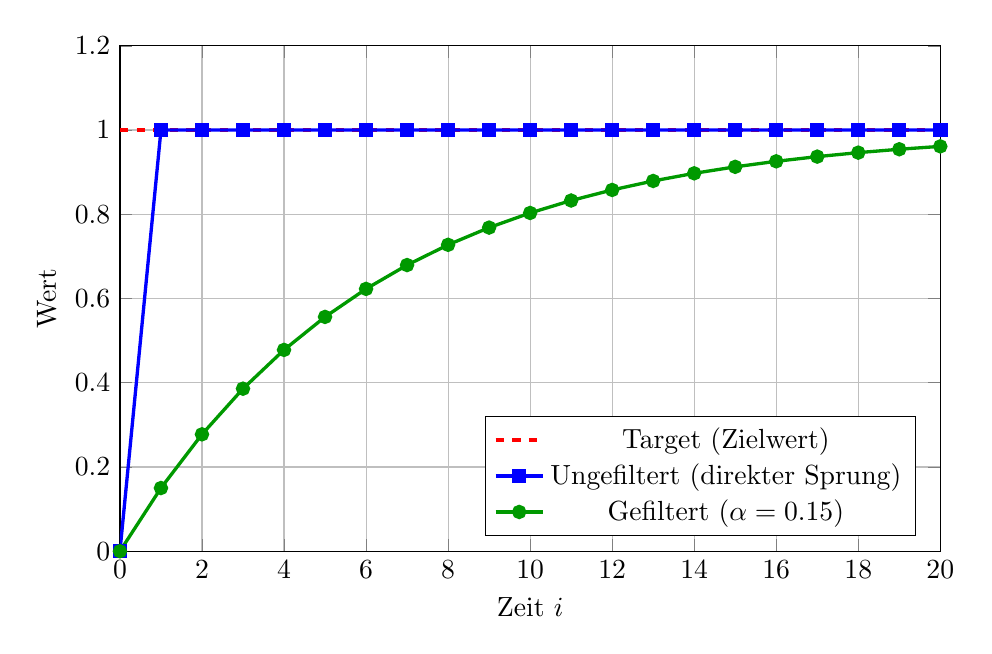
\begin{tikzpicture}
		
		% HIER ALPHA ÄNDERN!
		\def\alphaa{0.15}
		\def\numpoints{20}
		
		\begin{axis}[
			width=12cm,
			height=8cm,
			xlabel={Zeit $i$},
			ylabel={Wert},
			legend pos=south east,
			grid=major,
			ymin=0,
			ymax=1.2,
			xmin=0,
			xmax=\numpoints,
]
			
			% Zielwert (Target)
			\addplot[
			domain=0:\numpoints,
			samples=2,
			thick,
			dashed,
			red,
			line width=1.5pt
			] {1.0};
			\addlegendentry{Target (Zielwert)}
			
			% Ungefiltertes Signal (direkter Sprung)
			\addplot[
			mark=square*,
			blue,
			thick,
			line width=1.2pt,
			domain=0:\numpoints,
			samples=\numpoints+1
			] {x > 0 ? 1 : 0};
			\addlegendentry{Ungefiltert (direkter Sprung)}
			
			% Gefiltertes Signal - AUTOMATISCH BERECHNET!
			\addplot[
			mark=*,
			green!60!black,
			thick,
			line width=1.2pt,
			domain=0:\numpoints,
			samples=\numpoints+1
			] {x > 0 ? 1 - (1-\alphaa)^x : 0};
			\addlegendentry{Gefiltert ($\alpha = \alphaa$)}
			
		\end{axis}
		
%		% Formel Box
%		\node[align=left, fill=white, draw=black, thick, rounded corners] 
%		at (6, -1) {
%			\textbf{Filterformel:} \\
%			$\hat{X}_{i} = \hat{X}_{i-1} + \alpha (X_{i} - \hat{X}_{i-1})$ \\
%			mit $\alpha = \alpha$
%		};
		
	\end{tikzpicture}
